%!TEX root = ../../../report.tex
\section{Mechanics} % (fold)
\label{sec:mechanics}
This section deals with the mechanical design of the robot.
Based on the analysis performed in the chapter \ref{cha:analysis}, the mechancal design takes its results and carries out a specific analysis of each component.
Then, the conclusions are translated into a 3D model making a compromise between the requirements and manufacturability.

%!TEX root = ../../../../report.tex
\subsection{Motion transmission} % (fold)
\todo{Include a new section(?) detailing the implementation of the DD, SEA, PEA and SEA+PEA options}
\label{sub:pulleys_and_belts}
The section \ref{sec:joints} is dedicated to analyze and define what kind of motors and trasmision system is going to be used for each joint.
In the case of the knee and the ankle, the combination \textit{motor + gearbox + belt and pulleys} is chosen due to the preference of having the active actuator in the highest part of the link with the withdrawal of having to transfer the movement the lowest.
This system has been designed along with the torsional springs disussed in the section \ref{sub:compliance} where the rotation from the motor must feed the rotation of a serial rotational spring.
A system in which pulley and spring holder are joined, have to be done then.
The design of the pulley itself though, has been studied in terms of two factors: \textit{precision and backlash reduction} and \textit{integration with the serial rotational spring}.

\subsubsection{Precision and backlash reduction} % (fold)
\label{ssub:precision_and_backlash_reduction}
The goal of this design is to optimize the pulley in order to to get a lack of backlash.
Despite the platform is going to be used mainly for self-learning controllers (e.g. based on neuronal networks) and then the mechanical optimization is not a priority, the reduction of mechanical uncertainty is always good.

After analyze all the current solutions in the market, several non-backlash solutions are found.
Stands out the Gates GT3 Synchronous Belts \footnote{http://www.gates.com/products/industrial/industrial-belts/synchronous-belts/powergrip-gt3-belts} that is assured to be suitable for the presented application.
The withdrawals of this design are the lack of time for ordering such parts and the increase in the final price of the product. 
However there is another important factor, the integration that must be done with the serial rotational spring.
% subsubsection precision_and_backlash_reduction (end)

\subsubsection{Integration with the serial rotational spring} % (fold)
\label{ssub:integration_with_the_serial_rotational}
Another solution is to design and manufacture the pulley itself which would let to have a complete control of the design and manufacturability giving the possibility of integrate in a unique part design, the pulley for the transmission system and the spring holder.

At first, the GT3 design from Gates was intended to be designed.
However, its design is described in U.S. Patent Number 4,515,577, which doesn't allow its use.
Thus, the belts have been designed following the ISO 13050:2014 \cite{ISO13050} following the type T due to its focus in efficiency and reduction of backlash.
It is also appropriate for precision movements, high torques and low speeds, as our requirements.

The physical properties of the pulleys as the number of teeth, width, etc... have been chosen based on the ISO 5295:1987 \cite{ISO5295} and in sake of manufacturability.
As decided before, the pulley will belong to a part that will also have the task of holding the rotational serial spring.
This implies that the part will be designed to be 3D printed and thus, the criteria of design oriented to manufacturability must be applied.

Based on both ISO norms cited before and after some iterations based on experimental tests, the pulley T2,5 of 19 teeth gave the expected behavior.
Both pulleys are the same so no reduction is given from the motor shaft to he other.
In the figure \ref{fig:motor_pulley}, a detail of the designed pulleys can be seen.
% subsubsection integration_with_the_serial_rotational (end)

\subsubsection{Belts} % (fold)
\label{ssub:belts}
From \ref{ssub:integration_with_the_serial_rotational} a system pulleys-belt using T2,5 teeth profile was selected.
For the design of the belt system, an open belt whose initial tension can be adjusted with a zip-tie is chosen.
This allows to adjust the tension in any moment without increasing the costs plus it easy the maintenance.
No initial tensioning of the belts studies were carried out and it is expected that the user finds out the correct value by experimenting.
% subsubsection belts (end)

% subsection pulleys_and_belts (end)
%!TEX root = ../../../../report.tex
\subsection{Gears} % (fold)
\label{sub:gears}

\begin{figure}[ht!]
  \centering
  \includegraphics[width=0.5\textwidth]{figures/hip_gears}
  \caption{Teeth detail from pinion and gear.}
  \label{fig:teeth_detail}
\end{figure}

% subsection gears (end)
%!TEX root = ../../../../report.tex
\subsection{Impact force} % (fold)
\label{sub:impact_force}
In order to calculate the physical dimensions of some of the components, a bounding conditions have to be defined.
The presented case shows a peak of energy when landing after being jumped a estimated height.
This energy in then transmitted from the first contact point, the footprint, to the rest of the system, causing efforts that must be absorbed.
The components of the system must receive that energy under a controlled behavior -this is elastic deformations- assuring a longer life cycle of the legs.

Thus, some input parameters to calculate the impact force are assumed.
From this force will be sized all the consecutive components in the deformation chain.
Despite the deformation is of the whole system, the security coefficient assumed in here is going to be the calculation of all the components for that maximum force.

From the formula of the mechanical energy:
\begin{equation}
  E_{mechanical} = m g \Delta h + \frac{1}{2} m v^{2}
\end{equation}

The kinetic energy is negligible and only the energy form falling a certain height is supposed.
This energy is then translated into force by supposing a deformation of the whole body:
\begin{equation}
\label{eq:impact_force}
  F_{impact} = \frac{m g \Delta h}{t_{impact\_displacement}}
\end{equation}

The equation \ref{eq:impact_force} gives the force for sizing all the components.
Based on the input parameters defined in the appendix \ref{app:profile_selection} which are:
\begin{center}
\begin{tabular}{c | c}
  Parameter & Value \\
  \hline
  Total mass [kg] & 1.5 \\
  Jumping height [m] & 0.1 \\
  Impact displacement [m] & 0.005
\end{tabular}
\end{center}

The impact force is thus:
\begin{equation}
  F_{impact} = \frac{m g \Delta h}{t_{impact\_displacement}} = 294.40 N 
\end{equation}
% subsection impact_force (end)
%!TEX root = ../../../../report.tex
\subsection{Limb profile} % (fold)
\label{sub:limb_profile}
Based on the requirements of weight and its distribution defined in the analysis of the joints \ref{sec:joints}, the links have been decided to have in the upper extreme the motors. 
This leads to use a transmission system, such as belt and pulleys, which leaves for the rest of link an structural function that can also adopt the task of wiring placement.

Thus, a light weight section that satisfy the conditions of deformation and stress maximum will be chosen.
Carbon fiber is an ideal material to achieve this conditions of weight and stress so an quantitative analysis has been made calculating the optimal solution and then rounding it for all the possible profiles offered by the given provider.
The provider was chosen due to the previous experiences that the Mærsk Mc-Kinney Møller Institute had with carbon fiber orders.

The section profile offered \footnote{http://www.easycomposites.co.uk/\#!/cured-carbon-fibre-products/} are: \textit{Rod}, \textit{Tube}, \textit{Box}. The \textit{Stripe} and the \textit{Angle} are discarded due to its asymmetrical geometry that will will lead to less predictable scenarios.

  \subsubsection{subsubsection name} % (fold)
  \label{ssub:subsubsection_name}
  
  % subsubsection subsubsection_name (end)



% subsection limb_profile (end) 
%!TEX root = ../../../../report.tex

\subsection{Bearings} % (fold)
\label{sub:bearings}
In the section \ref{sub:impact_force} the force for sizing the bearings of the knee and the ankle was calculated.
The bearing elected would be such that allow dynamic loads of more than the impact force while keeping as small as possible to reduce the added weight to the robot.
On the other hand, the internal diameter comes defines by the rod diameter calculated in the section \ref{sub:rods}.

An estimation of nominal life of the bearing can be done from the Dynamic Load Rating (C), the Dynamic Equivalent Load (P) and the Life Rime Coefficient for a Ball Bearing (p) (being p=3 for balls bearings).
The equation \ref{eq:service_life_bearing}, shows the nominal life of one selected bearing \footnote{http://dk.rs-online.com/web/p/kuglelejer/8937420/}.
It is also worth to mention that the Dynamic Equivalent Load (P) is divided by the number of bearings in which the force is spread.
\begin{equation}
  \label{eq:service_life_bearing}
  L_{10} = \frac{10^{6}}{60 n} \left(\frac{C}{P}\right)^{p} = \frac{10^{6}}{60 n} \left(\frac{403}{294.4}\right)^{3} = 
\end{equation}

The term $L$ is the service life of a bearing (in number of hours or rpm), in normal conditions of speed and load, in which the bearing is working until fail by fatigue. 
Whilst $L_{10}$ is based in a stadistical model that is defined as the 90\% of the bearing of the same type will withstand those loads for a longer time.
% subsection bearings (end)
%!TEX root = ../../../../report.tex
\subsection{Rods} % (fold)
\label{sub:rods}
As explained in section \ref{sub:bearings}, it was decided to have two bearings per link (which gives four per joint) and a rod going through them.
This rod is then also used, in the case of the knee and the ankle, as a support for the pulleys that transmit the power from the motor to the next link.

Three mechanical efforts bound its design:
\begin{enumerate}
  \item \textbf{Shear strength}: in the case of the shear produced when an impact occurs and the rod of one link moves in the opposite direction than its relative in the consecutive link.
  \item \textbf{Resistance to bending}: due to the bending effort that the tension of the belt is constantly applying in the rod of the  knee and the ankle.
  \item \textbf{Torsion}: due to the pulley in the knee and the ankle. 
  This effort is negligible because zero-friction bearings are supposed.
\end{enumerate}

  \subsubsection{Shear analysis} % (fold)
  \label{ssub:shear_analysis}
  The maximum shear stress is found in the diameter of the cylinder (y=0) and is:
  
  \noindent\begin{minipage}{0.2\textwidth}% adapt widths of minipages to your needs
  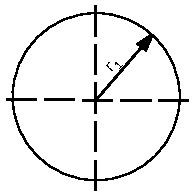
\includegraphics[width=\linewidth]{figures/profile_tube.pdf}
  \end{minipage}%
  \hfill%
  \begin{minipage}{0.8\textwidth}
    \begin{equation}
    \begin{aligned}
      \gamma_{yz} &= \frac{Q_y M_{x}^A*}{b(y) I_x} = \frac{Q}{r^2}\\
      M_{x}^{A_{y=0}} &= \frac{\pi r_1^2}{2} \\
      b(y=0) &= 2 r_1 \\
      I_x &= \frac{\pi r_1^4}{4}
      \end{aligned}
    \end{equation}
  \end{minipage}
  Given a tangent force Q, the shear stress can be calculated.
  If this is over the ultimate strength, the cylinder will break.
  % subsubsection shear_analysis (end)

  \subsubsection{Bending} % (fold)
  \label{ssub:bending}
  The bending analysis follows the one carried out in the section \ref{ssub:profile_study} for a cylinder.
  The equivalent force in this case is given by the tension of the belts, mainly the initial (though there are other tensions that appear when the belts moves for example).
  Due to feasibility reasons and the lack of the appropriate measurements devices, some experimental tests trying different tensions and axes where carried out giving good results with a 3 mm rod or more.
  % subsubsection bending (end)

  \subsubsection{Sizing} % (fold)
  \label{ssub:sizing}
  The studies above have been tested for different diameters of rod starting from the smallest size given by the provider and increasing until both conditions are satisfied, due to the requirements of weight reduction.
  In case of using steel as material, the ultimate strength is supposed to be 250 MPa\footnote{https://en.wikipedia.org/wiki/A36\_steel}.
  And for the case of a rod of 3 mm of diameter, both stresses are under the restrictions.
  Thus, 3 mm rods are going to be used.
  % subsubsection sizing (end)
% section rods (end)
%!TEX root = ../../../../report.tex

\subsection{Finite Element Method (FEM)} % (fold)
\label{sub:finite_element_method}
In the sections \ref{sub:limb_profile} and \ref{sub:rods}, pure mathematical tools have been used to calculate deformations and stresses.
This has been possible due to the simplification of the problem and the simple geometries found.
However, other parts have been analyzed with Finite Element Analysis (FEM), in which the part is subdivided into small volumes and then analyzed individually.
This allows the deformation and stress studies of complex geometries.

As an example, in the figures \ref{fig:fem_foot_iteration_1} and \ref{fig:fem_foot_iteration_2}, the iterative foot design is depicted.
Once the first iteration of the foot was modeled, the design has been changed in order to satisfy a minimum deformation criteria.
However, the designs have always been tested experimentally due to this analysis are under the assumption of isomorphic materials which, in the case of 3D printed parts like the shown in the figures, is not true.
The FEM studies have been used more as a qualitative analysis rather than quantitative.

\begin{figure}[ht]
    \centering
    \begin{subfigure}[b]{0.49\textwidth}
        \includegraphics[width=\textwidth]{figures/fem_5N_1.PNG}
        \caption{FEM analysis in left foot iteration 1}
        \label{fig:fem_foot_iteration_1}
    \end{subfigure}
    \begin{subfigure}[b]{0.49\textwidth}
        \includegraphics[width=\textwidth]{figures/fem_5N_2.PNG}
        \caption{FEM analysis in left foot iteration 2}
        \label{fig:fem_foot_iteration_2}
    \end{subfigure}
\end{figure}

% subsection finite_element_method (end)
%!TEX root = ../../../../report.tex
\subsection{Computer-Aided Design (CAD)} % (fold)
\label{sub:computer_aided_design}

\begin{figure}
    \centering
    \begin{subfigure}[b]{0.49\textwidth}
        \includegraphics[width=\textwidth]{figures/legs_foot.jpg}
        \caption{Left foot}
        \label{fig:left_foot}
    \end{subfigure}
    \begin{subfigure}[b]{0.49\textwidth}
        \includegraphics[width=\textwidth]{figures/legs_hip.jpg}
        \caption{Hip}
        \label{fig:hip}
    \end{subfigure}

    \begin{subfigure}[b]{0.49\textwidth}
        \includegraphics[width=\textwidth]{figures/legs_parts.jpg}
        \caption{Additional designed parts}
        \label{fig:mouse}
    \end{subfigure}
    \begin{subfigure}[b]{0.49\textwidth}
        \includegraphics[width=\textwidth]{figures/legs_pulley.jpg}
        \caption{Left ankle serial spring pulley}
        \label{fig:serial_spring_pulley}
    \end{subfigure}

    \begin{subfigure}[b]{0.49\textwidth}
        \includegraphics[width=\textwidth]{figures/legs_pulley_motor.jpg}
        \caption{Motor pulley}
        \label{fig:motor_pulley}
    \end{subfigure}
    \begin{subfigure}[b]{0.49\textwidth}
        \includegraphics[width=\textwidth]{figures/legs_knee_lower.jpg}
        \caption{Left lower knee}
        \label{fig:lower_knee}
    \end{subfigure}

    \begin{subfigure}[b]{0.49\textwidth}
        \includegraphics[width=\textwidth]{figures/legs_ankle_upper.jpg}
        \caption{Left upper ankle}
        \label{fig:ankle_upper}
    \end{subfigure}
    \begin{subfigure}[b]{0.49\textwidth}
        \includegraphics[width=\textwidth]{figures/legs_hip_lower.jpg}
        \caption{Left lower hip}
        \label{fig:hip_lower}
    \end{subfigure}

    \begin{subfigure}[b]{0.49\textwidth}
        \includegraphics[width=\textwidth]{figures/legs_hip_pinion.jpg}
        \caption{Hip's pinion}
        \label{fig:hip_pinion}
    \end{subfigure}
    \begin{subfigure}[b]{0.49\textwidth}
        \includegraphics[width=\textwidth]{figures/legs_knee_upper.jpg}
        \caption{Left upper knee}
        \label{fig:knee_upper}
    \end{subfigure}
\end{figure}

% subsection computer_aided_design (end)
%!TEX root = ../../../../report.tex
\subsection{Mechanical limits of the joints} % (fold)
\label{sub:mechanical_limits}
The implementation of mechanical limits for the joints obeys to two reasons:
\begin{enumerate}
  \item \textbf{Calibration}: they can be used as starting, known positions for the relative encoders.
  \item \textbf{Security}: a mechanical limit will restrict the movements and prevent any configuration non-natural or dangerous for the physical integrity of the robot.
\end{enumerate}

The Figure \ref{fig:joint_limits_hip} depicts how the mechanical limits of the hip (both left and right) are implemented in the upper part, comprising an angle of 90 + 60 = 150 degrees.
Figure \ref{fig:joint_limits_ankle_upper} shows the upper part of the ankle and how the allowed movement of the foot has a range of 60 + 50 = 110 degrees.
The mechanical limits of the knee are obtained as a combination of the lower and upper components of the joint.
These allow movements of 0 + 120 = 120 degrees as shown in the figures \ref{fig:joint_limits_knee_upper} and \ref{fig:joint_limits_knee_lower}.
The angles of the mechanical limits have been calculated according to the physical limitations in humans.

\begin{figure}[ht!]
    \centering
    \begin{subfigure}[b]{0.49\textwidth}
        \includegraphics[width=\textwidth]{figures/joint_limits_hip.PNG}
        \caption{Joint limits of the hip}
        \label{fig:joint_limits_hip}
    \end{subfigure}
    \begin{subfigure}[b]{0.49\textwidth}
        \includegraphics[width=\textwidth]{figures/joint_limits_ankle_upper.PNG}
        \caption{Joint limits of the ankle}
        \label{fig:joint_limits_ankle_upper}
    \end{subfigure}
\end{figure}    

\begin{figure}[ht!]
    \ContinuedFloat % continue from previous page
    \begin{subfigure}[b]{0.49\textwidth}
        \includegraphics[width=\textwidth]{figures/joint_limits_knee_upper.PNG}
        \caption{Joint limits of the knee: Upper link}
        \label{fig:joint_limits_knee_upper}
    \end{subfigure}
    \begin{subfigure}[b]{0.49\textwidth}
        \includegraphics[width=\textwidth]{figures/joint_limits_knee_lower.PNG}
        \caption{Joint limits of the knee: Lower link}
        \label{fig:joint_limits_knee_lower}
    \end{subfigure}
\end{figure}    

% subsection mechanical_limits (end)

% section mechanics (end)